% 
% Compile with ./build.sh
% 

\documentclass{beamer}

\usetheme{Madrid} 

%\usetheme{JuanLesPins}

\usepackage{listings}                                   
\usepackage{hyperref}
\usepackage{graphicx}                                 
\usepackage{tabularx}
\usepackage{microtype}
\usepackage[T1]{fontenc}
\usepackage[scaled]{beramono}
\usepackage{minted}
\usepackage{xcolor}
\usepackage{pgfplots}
\usepackage{dirtytalk}
\usepackage{tikz}
\usepackage{csquotes}
\usetikzlibrary{tikzmark,fit}

%\usepackage{enumitem}
\pgfplotsset{compat=1.6} 

\newcommand\Small{\fontsize{5}{5.2}\selectfont}
\newcommand*\LSTfont{\Small\ttfamily\SetTracking{encoding=*}{-60}\lsstyle}
\renewcommand{\footnotesize}{\tiny}

\hypersetup{colorlinks=color, linkcolor=black}
\definecolor{OliveGreen}{rgb}{0,0.6,0}
\graphicspath{{./images/}}
% 
% Turn off beamer nav stuff...
% 
\setbeamertemplate{navigation symbols}{}
\setbeamerfont{note page}{size=\tiny}

% 
% build with this option to only generate the notes
%
%\setbeameroption{show only notes}


%\input{lst-config/clojure-config}
\begin{document}

\begin{frame}
  \frametitle{Invest In Learning Immutable Tech}
  \center{
    %
    % Graphic for Title Page
    %
    
\includegraphics[scale=.15]{tech2}
    
  }
  \note{ Placeholder }
\end{frame}

\frame{
  \frametitle{Change is Inevitable}
  \huge
  \say{To improve is to change; to be perfect is to change often.}
  \large
  \rightline{{\rm  --- Winston Churchill}}
  \note{ Placeholder }
}

\frame{
  \frametitle{Change is Inevitable?}
  \huge
  \say{The more things change, the more they stay the same.}
  \large
  \rightline{{\rm  --- Jean-Baptiste Alphonse Karr}}
  \note{
    Developers are required to constantly learn new frameworks, platforms, 
    APIs, etc. However, so much of this is transient, eventually discarded outright or 
    replaced with something similar but new and shiny. There are many core tech components that 
    are virtually unchanging. Knowledge of these will be of value no matter your career path.
  }
}

\frame{
  \frametitle{Once Popular Tech}
   \begin{columns}
    \begin{column}{.49\textwidth}
      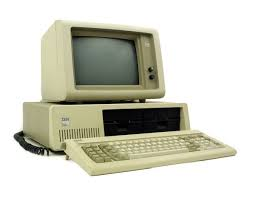
\includegraphics[scale=.50]{ibm-pc}
    \end{column}
    \begin{column}{.49\textwidth}
      \itemize{
        \item Adobe Flash
        \item Backbone
        \item COM
        \item CORBA
        \item DCOM
        \item Ember
        \item JEE (Websphere/Weblogic)
        \item JQuery
        \item Knockout
        \item SOAP
      }
    \end{column}
  \end{columns}
  \note{
    \begin{itemize}
      \item Common Object Request Broker Architecture
      \item COM/DCOM - Fear of Microsoft dominating the market at the time
      \item CORBA’s ultimate goal was to be a universal middleware standard for distributed, object-oriented computing—much like what web services, REST APIs, and gRPC 
            do today, but designed in an earlier era of computing.
      \item Flash - necessary in early days of web
      \item SOAP - Began as XML RPC - IBM and MS made it increasingly complex
      \item JEE - App Container ecosystem - multiple vendors implementing standards and competing
    \end{itemize}
  }
}

%\resetcounter[footnote]
%\setcounter{footnote}{0} 


%
% For databases, 
%
\frame{
  \frametitle{Database}
  \begin{columns}
    \begin{column}{.49\textwidth}
      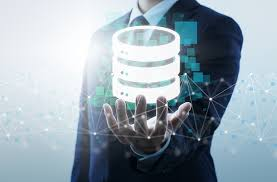
\includegraphics[scale=.615]{db}
      \vfill
      
\includegraphics[scale=.62]{sql}  
    \end{column}
    \begin{column}{.49\textwidth}
      \itemize{
      \item Postgres
      \item SQL Server
      \item Oracle
      \item SQLite
      \item Couchbase
      \item Cassandra
      \item DynamoDB
      \item Bigtable
      \item Snowflake
      \item DB2
      \item H2
      \item MySQL
      }

    \end{column}
  \end{columns}
  \note{
    \begin{itemize}
      \item Processing data is the essence of computing
      \item Application stacks come and go, but data can live forever. In some cases, the older the data
            the more valuable it is.
      \item The native language of most databases is some form of SQL.
      \item NOSQL - better name is Not Relational or No Joins
      \item stack-overflow (SQL Server) and wikipedia (mariaDB) as examples where 
      relational can be web scale
      \item Postgres wire protocol is becoming a defacto integration protocol for data
      \item utillity of H2 beyond tests - server mode, limited cluster ability, 
      great for slurping CSV data for SQL hacking
      \item H2 supports postgres wire protocol, facilitating using H2 with languages other
      than java
      \item H2 great for small apps - I use it for storing logs on apps that run on raspbery pi.
            Using a DB client + SQL is very useful for looking at your logs.
    \end{itemize}
  }
}

\frame{
  \frametitle{Operating Systems}
  \begin{columns}
    \begin{column}{.49\textwidth}
      
\includegraphics[scale=.13]{operating-systems}
    \end{column}
    \begin{column}{.49\textwidth}
      \itemize{
      \item Trouble Shooting
      \item Debugging
      \item Performance Tuning
      \item Productivity
      %  \footnote{\href{https://www.ics.uci.edu/~lopes/teaching/inf212W12/readings/church.pdf}
      %    {An Unsolvable Problem of Elementary Number Theory}}
      }

    \end{column}
  \end{columns}
  % \center{
  %   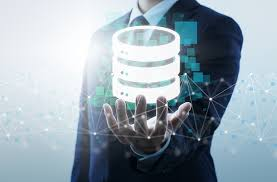
\includegraphics[scale=.75]{db}
  \note{ TODO }
  }

  \frame{
  \frametitle{Operating System Foundations}
  \begin{columns}
    \begin{column}{.49\textwidth}
      
\includegraphics[scale=.13]{operating-systems}
    \end{column}
    \begin{column}{.49\textwidth}
      \itemize{
      \item Shared Memory
      \item Semaphores
      \item Processes
      \item Threads
      \item Device Drivers
      \item Kernel vs User Space
      \item Sockets
      \item Pipes
      \item File Systems
      }

    \end{column}
  \end{columns}
  \note{ 
    \begin{itemize}
      \item These are the core concepts that underly most operating systems
      \item Even if you are not doing systems programming, these concepts will come up frequently
            in many contexts, including trouble shooting.
      \item Even if you stay in higher-level application development, 
            having \enquote{systems intuition} sets you apart
      \item It makes you better at reading tools like top, htop, strace, 
            vmstat, or Windows Performance Monitor
    \end{itemize}  
   } 
  }

% \frame{
%   \frametitle{Title - Page of Items}
%   \begin{itemize}
%   \item Item 1
%   % To not show following item until keypress
%   % \pause
%   \item Item 2
%   \item Item 3
%   \end{itemize}
% }




  \frame{
    \frametitle{Networking}
    \begin{columns}
      \begin{column}{.49\textwidth}
        
\includegraphics[width=0.90\textwidth]{networking}
      \end{column}
      \begin{column}{.49\textwidth}
        \itemize{
          \begin{small}
            \item TCP Transmission Control Protocol
            \item UDP User Datagram Protocol
            \item HTTP Hypertext Transfer Protocol
            \item SFTP Secure File Transfer Protocol
            \item SSL Secure Socket Layer
            \item DHCP Dynamic Host Configuration Protocol 
            \item DNS Domain Name System
            \item SMTP Simple Mail Transfer Protocol
            \item IMAP Internet Message Access Protocol
            \item POP3 Post Office Protocol 3
        % {\href{https://www.rfc-editor.org/rfc-index.html}
        % {RFC Index}}
          \end{small}
        }
      \end{column}
    \end{columns}
    % \center{
    %   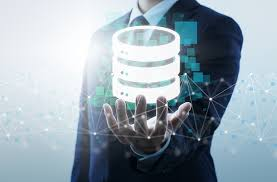
\includegraphics[scale=.75]{db}
    \note { 
      \begin {itemize} 
      \item The protocols here define the foundation for how humanity (and machines)
           communicate digitally
      \item These protocols are stable and have been in use for decades
      \item TCP - 1974 RFC 675 
      \item UDP - 1980 RCF 768
      \item SMTP - 1982 RFC 821
      \item DNS - 1983 RFC 882,883
      \item HTTP - 1991 RFC 1945
      \item SSL - 1995 RFC 6101
      \item No matter what type of software dev you are engaged in, details of these protocols
            will arise frequently in many contexts, especially troubleshooting.
      \end {itemize}
    }  
  }
 
\frame{
    \frametitle{CLI Tools}
    \begin{columns}
      \begin{column}{.49\textwidth}
        
\includegraphics[width=0.90\textwidth]{bash}
      \end{column}
      \begin{column}{.49\textwidth}
        \itemize{
        \item sh/bash
        \item awk
        \item sed
        \item find
        \item grep
        \item netstat
        \item screen
        \item nohup
        \item od
        \item strings
        \item objdump
        }
      \end{column}
    \end{columns}  
    \note{
      \begin{itemize}
        \item sh/bash - Yes, there are other more popular shells, but sh/bash is almost always 
              available in all unix environments
        \item Even if you don't like unix shell scripting, there will always be production support
              issues arise where you need to do something quickly. Knowing sh scripting to an 
              intermediate level will serve you well
        \item WSL - Windows Subsytem for Linux - bash on windows
      \end{itemize}
     }
    }

    \frame{
    \frametitle{JVM Internals}
    \begin{columns}
      \begin{column}{1\textwidth}
        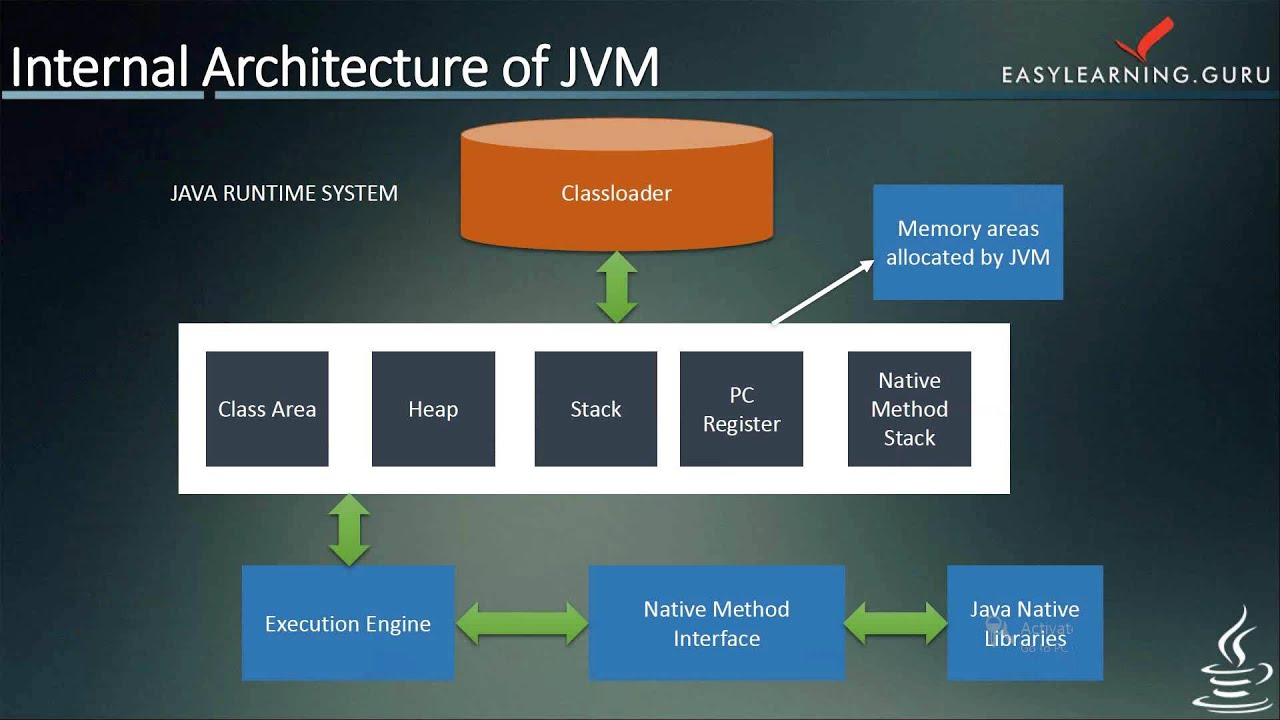
\includegraphics[width=0.90\textwidth]{jvm-internals}
      \end{column}
    \end{columns}
    \note{
      \begin{itemize}
        \item jps
        \item jstack
        \item jmap
        \item jcmd
        \item visulVM
      \end{itemize} 
      }
    }

    \frame{
    \frametitle{JVM - Not Limted to Java the Language}
    \begin{columns}
      \begin{column}{.49\textwidth}
        
\includegraphics[width=0.90\textwidth]{jvm}
      \end{column}
      \begin{column}{.49\textwidth}
        \itemize{
        %\pause
        \item Kotlin
        %\pause
        \item Scala
        %\pause
        \item Groovy
        %\pause
        \item JRuby
        %\pause
        \item Clojure
        }
      \end{column}
    \end{columns} 
    \note{
      \begin{itemize}
        \item Kotlin - a better java
        \item Groovy - adds more dynamic behavior to java
        \item JRuby - is a good source of info regarding details of what is happening in the JVM internals
        \item Clojure - functional lisp, excellent java interop - greatest hits of comp sci from last 50 years
      \end{itemize}
     }
   }
  

\frame{
  \frametitle{Resources}
  \begin{itemize}

  \item \href {https://www.rfc-editor.org/rfc-index.html}{\color {blue}{RFC Index}}
  %\item \href {https://developer.arm.com/documentation/107829/0200/Assembly-language-basics}{\color {blue}{ARM Assembly Language}}
  \item \href {https://www.youtube.com/watch?v=OT1RErkfLNQ}{\color {blue}{SQL - Beginner to Advanced in 4 hours}}
  %\item \href {https://os.ecci.ucr.ac.cr/slides/Abraham-Silberschatz-Operating-System-Concepts-10th-2018.pdf}{\color {blue}{Operating System Concepts}}
  \item \href {https://www.geeksforgeeks.org/operating-systems/operating-systems}{\color {blue}{Operating System Tutorial}}
  %\item \href {https://www.clojure.org}{\color {blue}{Clojure}}
  \item \href {https://datastation.multiprocess.io/blog/2022-02-08-the-world-of-postgresql-wire-compatibility.html}{\color {blue}{Postgres Wire Protocol}}
  \item \href {https://www.clojure.org}{\color {blue}{Clojure}}
  \item \href {https://www.jruby.org}{\color {blue}{JRuby}}
  \item \href {https://kotlinlang.org/spec/introduction.html}{\color {blue}{Kotlin}}
  \item \href {https://www.youtube.com/watch?v=zWVV31NYi1U}{\color {blue}{Bash Tutorial}}
  \item \href {https://learn.microsoft.com/en-us/windows/wsl/about}{\color {blue}{WSL - Windows Subsystem for Linux}}
  \item \href {https://clojure.org/api/cheatsheet}{\color {blue}{Cheatsheet Tool}}
  
  \item \href {https://github.com/tstout/presentations/blob/main/immutable-tech/immutable-tech.tex}{\color {blue}{Source Code For This Document}}
  \end{itemize}
  \note{ Placeholder }
}

\end{document}
